\documentclass[a4paper,11]{article}

%\title{Unused Title}
\usepackage{graphicx}
\usepackage{hyperref}
\usepackage{multirow}
\usepackage{multicol}
\usepackage{blindtext}
\usepackage[utf8]{inputenc}
\usepackage[english]{babel}
\usepackage[T1]{fontenc}
\usepackage{natbib}

% Use helvet if uarial cannot be installed
%\usepackage{uarial}
\usepackage[scaled]{helvet}

\renewcommand{\familydefault}{\sfdefault}
\usepackage{fixltx2e}
\usepackage{amssymb}
\usepackage{amsmath}
\usepackage{courier}
\usepackage{setspace}
\usepackage{lineno}
\usepackage[table,svgnames]{xcolor}
\usepackage{fancyvrb} 
\usepackage{listings}
\usepackage{caption}
\usepackage{longtable}
\usepackage{relsize}
\usepackage{tfrupee}
\usepackage{rotating}
\usepackage{lipsum}
\usepackage{subcaption}
\usepackage{float}
\usepackage{aliascnt}
\usepackage{pdfpages}
\usepackage{graphicx}
\usepackage{natbib}
\usepackage{caption}
\captionsetup{
  compatibility = false
}
\newcommand*{\urlprefix}{Available from: }
\newcommand*{\urldateprefix}{Accessed }
\bibliographystyle{bath}
\renewcommand{\bibsection}{}

\makeatletter
\newcommand\footnoteref[1]{\protected@xdef\@thefnmark{\ref{#1}}\@footnotemark}
\makeatother

\newaliascnt{eqfloat}{equation}
\newfloat{eqfloat}{h}{eqflts}
\floatname{eqfloat}{Equation}

\newcommand*{\ORGeqfloat}{}
\let\ORGeqfloat\eqfloat
\def\eqfloat{%
	\let\ORIGINALcaption\caption
	\def\caption{%
		\addtocounter{equation}{-1}%
		\ORIGINALcaption
	}%
	\ORGeqfloat
}

\addto\captionsenglish{% Replace "english" with the language you use
	\renewcommand{\contentsname}%
	{List of Contents}%
}

\newcommand\tab[1][1cm]{\hspace*{#1}}

\definecolor{codegreen}{rgb}{0,0.6,0}
\definecolor{codegray}{rgb}{0.5,0.5,0.5}
\definecolor{codepurple}{rgb}{0.58,0,0.82}
\definecolor{backcolour}{rgb}{0.95,0.95,0.92}

\lstdefinestyle{mystyle}{
	backgroundcolor=\color{backcolour},   
	commentstyle=\color{codegreen},
	keywordstyle=\color{magenta},
	numberstyle=\tiny\color{codegray},
	stringstyle=\color{codepurple},
	basicstyle=\ttfamily\footnotesize,
	breakatwhitespace=false,         
	breaklines=true,                 
	captionpos=b,                    
	keepspaces=true,                 
	numbers=left,                    
	numbersep=5pt,                  
	showspaces=false,                
	showstringspaces=false,
	showtabs=false,                  
	tabsize=2,
	xleftmargin=0.5cm,
	xrightmargin=-0.8cm,
	frame=lr,
	%	framesep=-5pt,
	framerule=0pt
}

\lstset{style=mystyle}

\definecolor{Teal}{RGB}{0,128,128}
\definecolor{NewBlue1}{RGB}{4,100,226}
\definecolor{NiceBlue}{RGB}{63,104,132}
\definecolor{DarkRed}{RGB}{14,53,59}
\definecolor{NewBlue2}{RGB}{62,100,125}
\definecolor{NewBlue3}{RGB}{44,100,128}

\hypersetup{
	colorlinks,
	citecolor=NiceBlue,
	linkcolor=NewBlue1,
	urlcolor=Blue
	%	citebordercolor=Violet,
	%	filebordercolor=Red,
	%	linkbordercolor=Blue
}

\usepackage{geometry}
\linespread{1.25}
\usepackage[parfill]{parskip} % Avoid indentation

\geometry{
	a4paper,
	left=2cm,
	right=2cm,
	top=2cm,
	bottom=2cm,
}
\onehalfspacing
\linenumbers

% -------- Fancy page headers:
\usepackage{fancyhdr}
\pagestyle{fancy}
\fancyhf{}
\rhead{\slshape\nouppercase\leftmark}
\lhead{\slshape\nouppercase{\rightmark}}
\renewcommand{\headrulewidth}{1pt}
\renewcommand{\footrulewidth}{1pt}

\lfoot{\thepage}
\rfoot{\thepage}

\begin{document}
	\begin{center}
		{\large IMPERIAL COLLEGE LONDON SILWOOD CAMPUS}
	\end{center}
	%	\maketitle
	\vspace{3cm}
	
	\begin{center}
	\title{\line(1,0){250}\\ \Huge \textbf{The Domestication and Natural History of Horses: a Genomic Approach}\\ \line(1,0){250}}	
		\Huge \textbf{The Domestication and Natural History of Horses: a Genomic Approach}\\		
		\vspace{1cm}		
		
	\end{center}
	\vspace{2cm}
	\begin{center}
	
		\LARGE \textbf{Maddalena Cella}\\ \Large mc2820@ic.ac.uk\\
		\vspace{3cm}
		\end{center}
		\Large \textbf{Main Supervisor}: Dr Matteo Fumagalli, m.fumagalli@imperial.ac.uk\\
		\Large \textbf{Co-supervisor}: Prof Vincent Savolainen, v.savolainen@imperial.ac.uk \\

	
	\vspace{5cm}
	
		{\large \textbf{keywords:} bioinformatics, genomics, direct to consumer genetics, population genetics, domestication, animal agriculture }

	\newpage

\cleardoublepage\pagenumbering{arabic}

\section{Introduction}
    Direct-to-consumer genetic (DCTG) tests allow individuals to obtain information regarding ancestry and other traits of interest at a low cost. DTCG is normally used in humans, but has been recently introduced for domestic animals such as cats and dogs \citep{DTCcats, DTCdogs}. Animal agriculture is another area that could benefit from DTCG as it allows breeders to have easy access to health and disease information about individuals at a low cost. DTCG normally uses Single Nucleotide Polymorphism (SNP) arrays to target SNP associated with traits of interest \citep{khan2018consumer}, however when a good reference panel is available, low coverage Whole Genome Sequencing (WGS) could have a similar performance to SNP arrays. 
    Recent improvements in horse genomics include the release of a new improved horse reference genome assembly (EquCab3.0) \citep{horserefgenome, Equ-Cab3.0}. The high quality of the assembly has allowed the development of SNP arrays and WGS of thousands of individual horses and the identification of many SNPs related to health and performance \citep{horserefgenome}.
    Given the amount genome data available for horses and the interest in them for entertainment, agriculture and the petting industry, they represent the ideal species for testing the use of low-coverage WGS to infer ancestry and phenotype traits of interest. In particular, having at my disposal a hair DNA sample from a mixed-breed horse sequenced at low-coverage, I aim to:\newline
    1. predict its ancestry from a reference panel of horses breeds; \newline
    2. predict its phenotype for some traits of interest; \newline
    3. write a comprehensive pipeline for the workflow used to achieve 1. and 2.

\section{Methods}
    I will obtain WGSs from NCBI and ENA to create a reference panel of horse breeds. The DNA sample of a mixed-breed horse sequenced at low-coverage will be mapped against the reference panel to infer ancestry and individual admixture levels. I will also infer the phenotype of the sample by looking at the presence or absence of SNPs associated with some Mendelian traits of interest \citep{horserefgenome}. In order to infer ancestry and phenotype, I will utilise a variety of scripts and programmes already available, as well as develop new tools when necessary. 
    The pipeline developed will be written in \textit{Nextflow}, which ensures reproducibility of the analysis by avoiding numerical instability through multi-scale containerisation \citep{nextflow}.

\section{Anticipated Outputs and Results}
    I expect to successfully infer ancestry and admixture levels of the mixed-breed sample as well as its phenotype for some Mendelian traits of interest. I also anticipate the development of a reproducible and comprehensive workflow for the use of low-coverage WGS in replacement of SNP arrays for DCTG.
\section{Budget}
    The project as described above does not require additional costs.
\section{Project Feasibility}
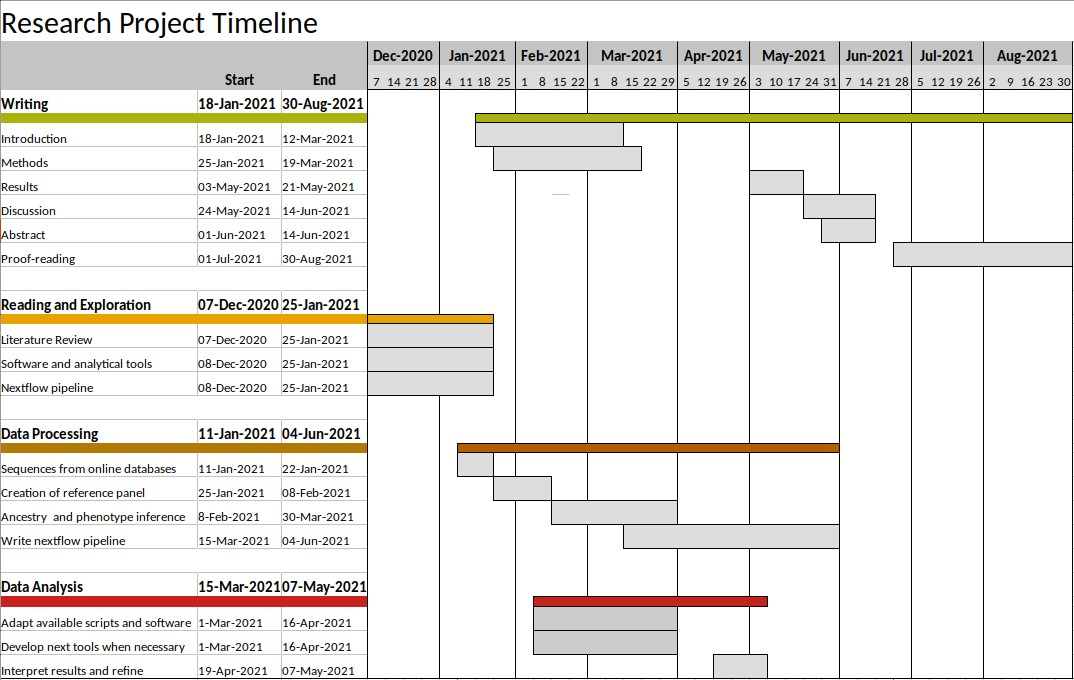
\includegraphics[width=\textwidth]{ciao.jpg}

\pagebreak

\section{References}
\bibliography{references.bib}
\pagebreak

I have seen and approved the proposal and the budget.\newline\newline
Dr. Matteo Fumagalli, 18/12/2020.\newline

\includegraphics[scale=0.5]{signature.png}
\end{document}          
